\documentclass[11pt,a4paper,titlepage]{article}

\usepackage{pdflscape}
\usepackage[margin=1in]{geometry}
\usepackage{titling}
\usepackage{graphicx}
\usepackage{subcaption}
\usepackage{titlesec}
\usepackage{datetime}
\newcommand{\sectionbreak}{\clearpage}
\usepackage[hidelinks]{hyperref} 

\graphicspath{ {./Images/} }

\setcounter{secnumdepth}{4}

\titleformat{\paragraph}
{\normalfont\normalsize\bfseries}{\theparagraph}{1em}{}
\titlespacing*{\paragraph}
{0pt}{3.25ex plus 1ex minus .2ex}{1.5ex plus .2ex}

\newdateformat{monthyeardate}{%
  \monthname[\THEMONTH], \THEYEAR}

\begin{document}
%\title{ \huge Functional Requirements for the SAMBUG}

\begin{titlepage}
	
	
	\begin{center}
		\vspace*{-3cm}
  		\makebox[\textwidth]{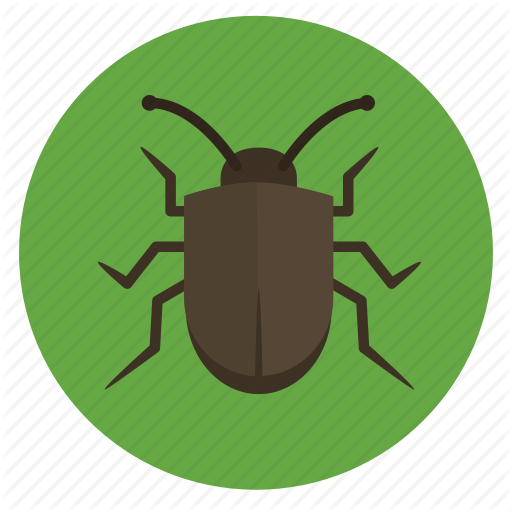
\includegraphics[width=\paperwidth]{sambug}}
	\end{center}
	
	%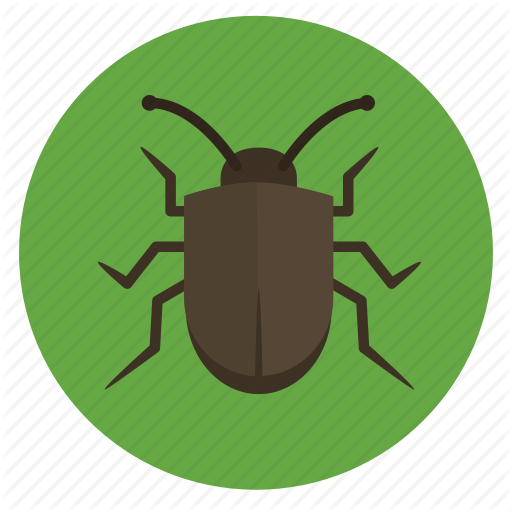
\includegraphics[width=\paperwidth]{sambug}
	
    \vspace*{2cm}
      \Huge \textbf {SAMBUG}\\
      
    \vspace*{-0.5cm}
	  \huge \textbf {User Manual}\\
	  
	\vspace*{-0.5cm}  
      \LARGE \textbf {Subtrop}
         
    \vskip2cm
          
    \large \textbf{\monthyeardate\today}
  
    \vfill
\end{titlepage}
	
	

\tableofcontents
\listoffigures

\pagebreak

\section{System Overview}
\subsection{Introduction}
SAMBUG is a system that will ease the process of stinkbug pest scouting on a farm. Features of the system include stinkbug classification and recognition, data storage, reporting on various scouting trips and more.
\subsection{Utilisation}
Farmers can use the system in two ways, namely an Android application and a browser interface.\\\\
The way in which the system will help farmers will be listed below:
	\begin{itemize}
		\item Farmers can easily use the Android application to classify stink bugs (during a scouting trip). Classification can be done using two methods, manual classification and automatic classification:
		\begin{itemize}
			\item \textbf{Manual Classification:} This method allows the user to take a photo of a single bug and compare it with various other photos taken from a pre-selected gallery of photos. The user will select the photo that most resembles the bug that he/she wants to classify.
			\item \textbf{Automatic Classification:} This method also allows the user to take a photo of the specific bug, and thereafter the application will do the classification by using an artificially intelligent system. 
		\end{itemize}
		\item While scouting and classifying bugs, the application makes it easy to enter additional data, such as the number of that specific bug that was found, in which block of the farm it was, etc.
		\item After doing a scout trip, a summary will be shown, summarising the number and types of bugs found during that trip. Using this summary, farmers can decide with more confidence if spraying pesticide is necessary or not.
		\item When taking a photo during classification, the geolocation will be taken as well. With this feature, farmers will find it easier to make sure that scouts actually go out to random locations.
		\item After capturing the data for a scout trip, this data will be stored in a database such as to later look back at the data.
		\item The browser interface will offer various services, of which the most important is reporting services based on previous scouting trips.
		\item Administrators at Subtrop will be able to view data from different farms to also help them reach conclusions.
		\item On the browser interface it will be possible to enter data concerning pesticide spraying. This will also be stored in the database and may later be used to view data.
	\end{itemize}
	
\subsection{Intended Audience}
The intended audience of this systems is farmers specifically dealing with stink bugs as pests on their farms. Any farmer who seeks assistance with regards to bug classification, data management and scout trip management will find the system useful. The system will specifically assist farmers who do scouting of pests to reach certain conclusions, such as whether to spray pesticide or not, where and when pests are more, etc.

\subsection{Users}
The system has in mind three different users which will be described bellow:
	\begin{itemize}
		\item \textbf{Staff of Subtrop} These users will have access to all data from all the farms using the system. This means that when they log on in the browser interface they will be able to generate reports based on collective data from all farms.
		\item \textbf{Farmers} Farmers will use the browser interface, but may also use the Android application. Farmers will only be able to generate reports based on data from their own farm, thus other farms' data will not be visible. 
		\item \textbf{Scouts} Scouts will mainly use the Android Application to enter data and do classifications while in the field. The Android application is developed to keep in mind different language preferences, thus minimum usage of actual words and more symbols to carry over a message.
	\end{itemize}



\section{System Configuration}
Before we go into any further detail, it is important to ensure that you are fully equipped with the necessary prerequisites to enjoy the SAMBUG system. This section outlines everything you need to get started.
\subsection{Setup Overview}
SAMBUG is intended to be an integrated solution. The Android application and Website are complementary. Figure \ref{fig:layout} depicts the common high-level configuration of the system. Please note that Figure \ref{fig:Web} may be interchanged with any Web-enabled device.
	\begin{figure}[h]
		\begin{subfigure}{0.3\textwidth}
			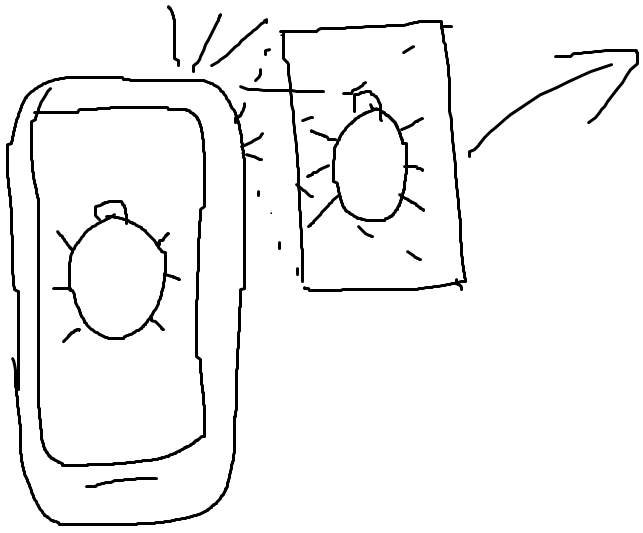
\includegraphics[width=0.9\linewidth]{Fig1a}
		\caption{Data Capture}		
		\label{fig:dataCapt}	
		\end{subfigure}
		\begin{subfigure}{0.3\textwidth}
			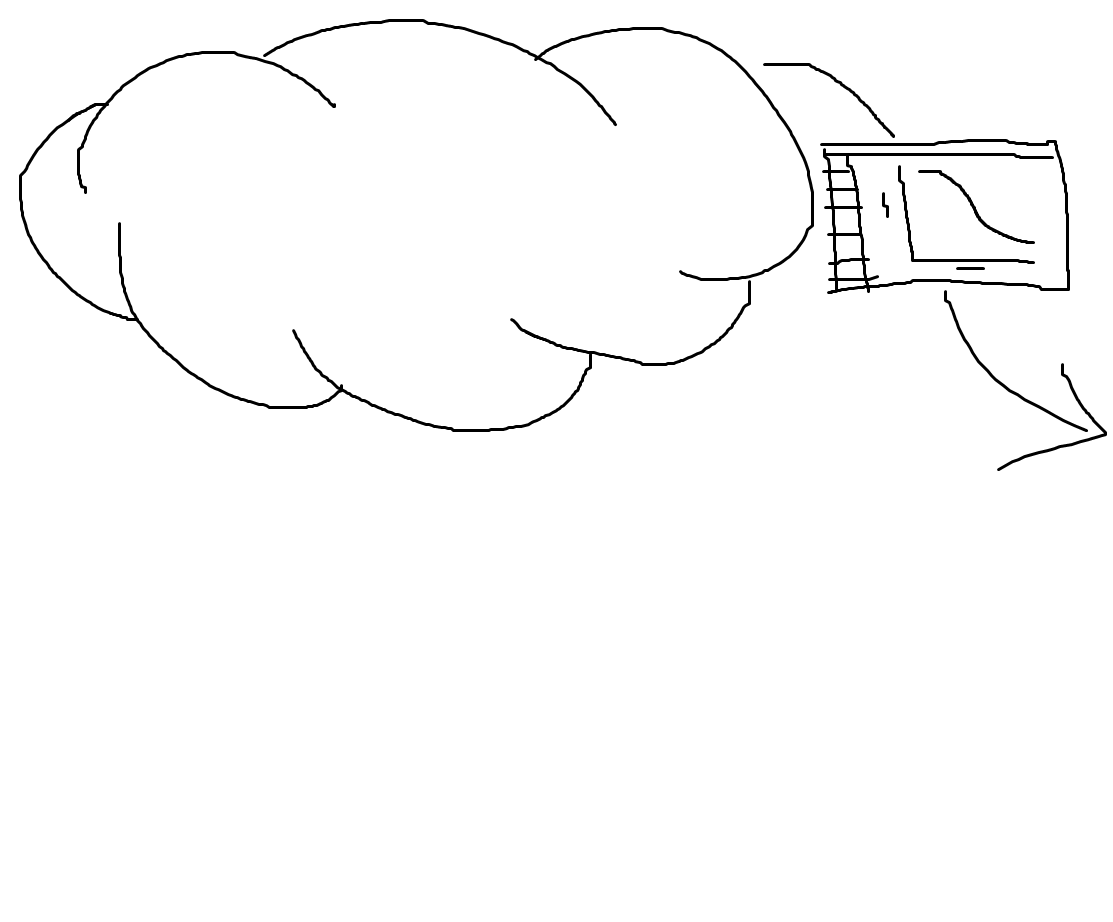
\includegraphics[width=0.9\linewidth]{Fig1b}
		\caption{History \& Analysis}		
		\label{fig:Engine}	
		\end{subfigure}
		\begin{subfigure}{0.3\textwidth}
			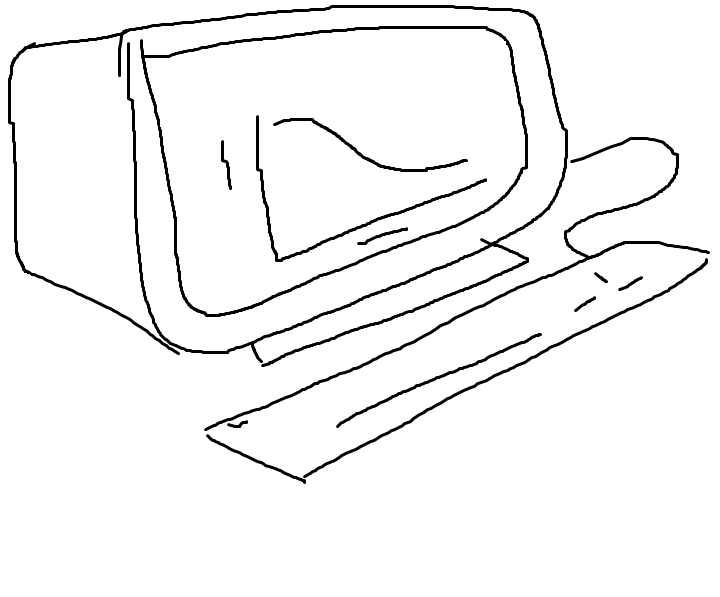
\includegraphics[width=0.9\linewidth]{Fig1c}
		\caption{Farm Management \& Consolidation}	
		\label{fig:Web}		
		\end{subfigure}
	\caption{Illustration of SAMBUG's Configuration}
	\label{fig:layout}
	\end{figure}

\subsection{Hardware \& Software Requirements}
The design of the system as indicated above lends itself to a number of required devices and services, including:
	\begin{itemize}
		\item An Android Smartphone or Tablet \footnote{You are advised to use a device with a camera that's able to take good quality macro photos in a medium level of light} (Android 4.1 or higher) - This will house the application used during Scouts, your main access point to the system.
		\item A Second Web-enabled device - This is where you will manage your farm and view consolidated information of your scouts. Although you may choose to use the same phone/tablet you use in the field, the Web-based nature of this part of the system will allow you to work on a device with a large display, suitable for office work (e.g. a PC).
		\item An Internet Browser - Whatever your choice of device in Figure \ref{fig:Web}, it must have one or more of the latest (As of \monthyeardate\today) popular Internet Browsers installed. You may choose from an extensive list, including, but not limited to:
		\begin{itemize}
			\item Google Chrome
			\item Internet Explorer/Microsoft Edge
			\item Mozilla Firefox
			\item Safari
		\end{itemize}
		\item An Internet Connection - Our application is designed to perform all of its functions even where no mobile/WiFi network reception is available. However, the information you'll be gathering during your scouting trips will have to be uploaded to the server at some point, and for that, you need to be connected to the internet. 		
	\end{itemize}



\section{Installation}
The Android application will be available for download via the Google Play store (in the future). The web application will be permanently available via the internet.
		
\section{Getting started}
\subsection{Requirements to access the system}
For a user to use the system, it is necessary that he/she registers as a user first. This can only be done on the web page. Only an email address, password and farm name will be asked for at registration. All users are automatically 'normal' users, that is users who do not have the authority of seeing all farms' data (such as Subtrop staff). A user can only become a privileged user if another privileged user authorises him/her. Farmers and scouts will use the same account, and thus the same credentials to use the system.\\
After registration the user can log in on the Android Application as well as the web page. A user logged in to the Android application will stay logged in if he/she does not explicitly log out. The details used to log in are only the email (as a username) and password.

\subsection{A walk through the system}

%INFORMAL IDEAS

The main flow of the system:\\
\begin{itemize}
\item On the Application: 
	\begin{itemize}
		\item Login
		\item Enter the scouting data
	\end{itemize}
\item Web Page
	\begin{itemize}
		\item Register on browser interface.
		\item Add for the first time all the blocks currently on the farm.
		\item Log On to browser interface.
		\item View reports on historical data. There are various reporting mechanisms,such tables, maps and graphs. Each of these mechanisms will allow filters to be applied to only view specific data.
\item Enter treatment data if pesticide was sprayed.
	\end{itemize}
\end{itemize}


Other aspects:\\
May change profile settings, may CRUD blocks also.\\\\

If the user is a subtrop staff member, they will not use the app, but only the web interface. Will also not enter any data. Will only view data.\\

Thus work flow may differ for different users.



\section{Using the System}
\subsection{Web Page}
		 To be continued...
\subsection{Android Application}
	The application functions as a simple way for scouters to enter data. Follow these steps in order to use the application for scouting:
	\begin{enumerate}
		\item Open the application by clicking on the SAMBUGApp icon on your Android Device
		\item Once the Application has succesfully been opened please login in with your registered username and password. If you have not yet registered please go to the web page as described in the previous section in order to register. Click on Sign In to continue.
			\begin{center}
				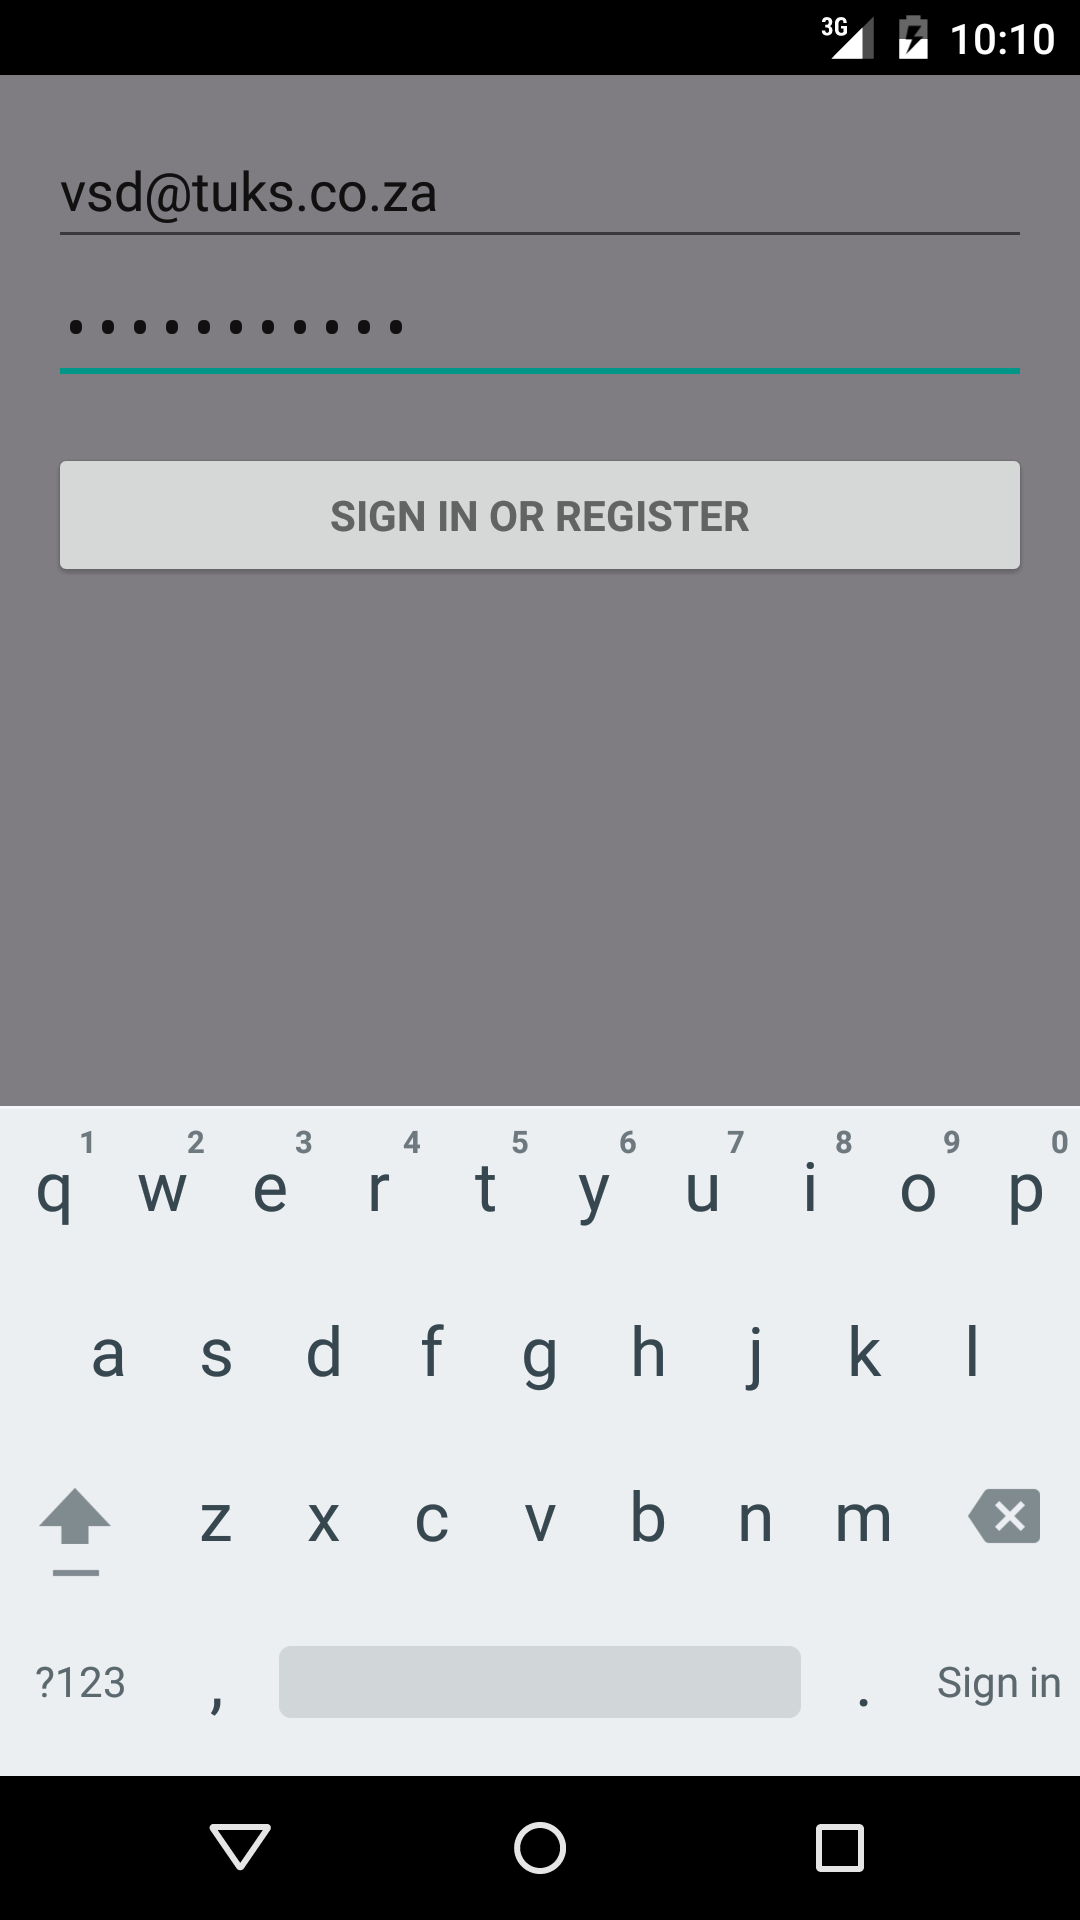
\includegraphics[scale=0.13]{shot1}
			\end{center}
		\item After successful login you will be presented with the following screen:
			\begin{center}
				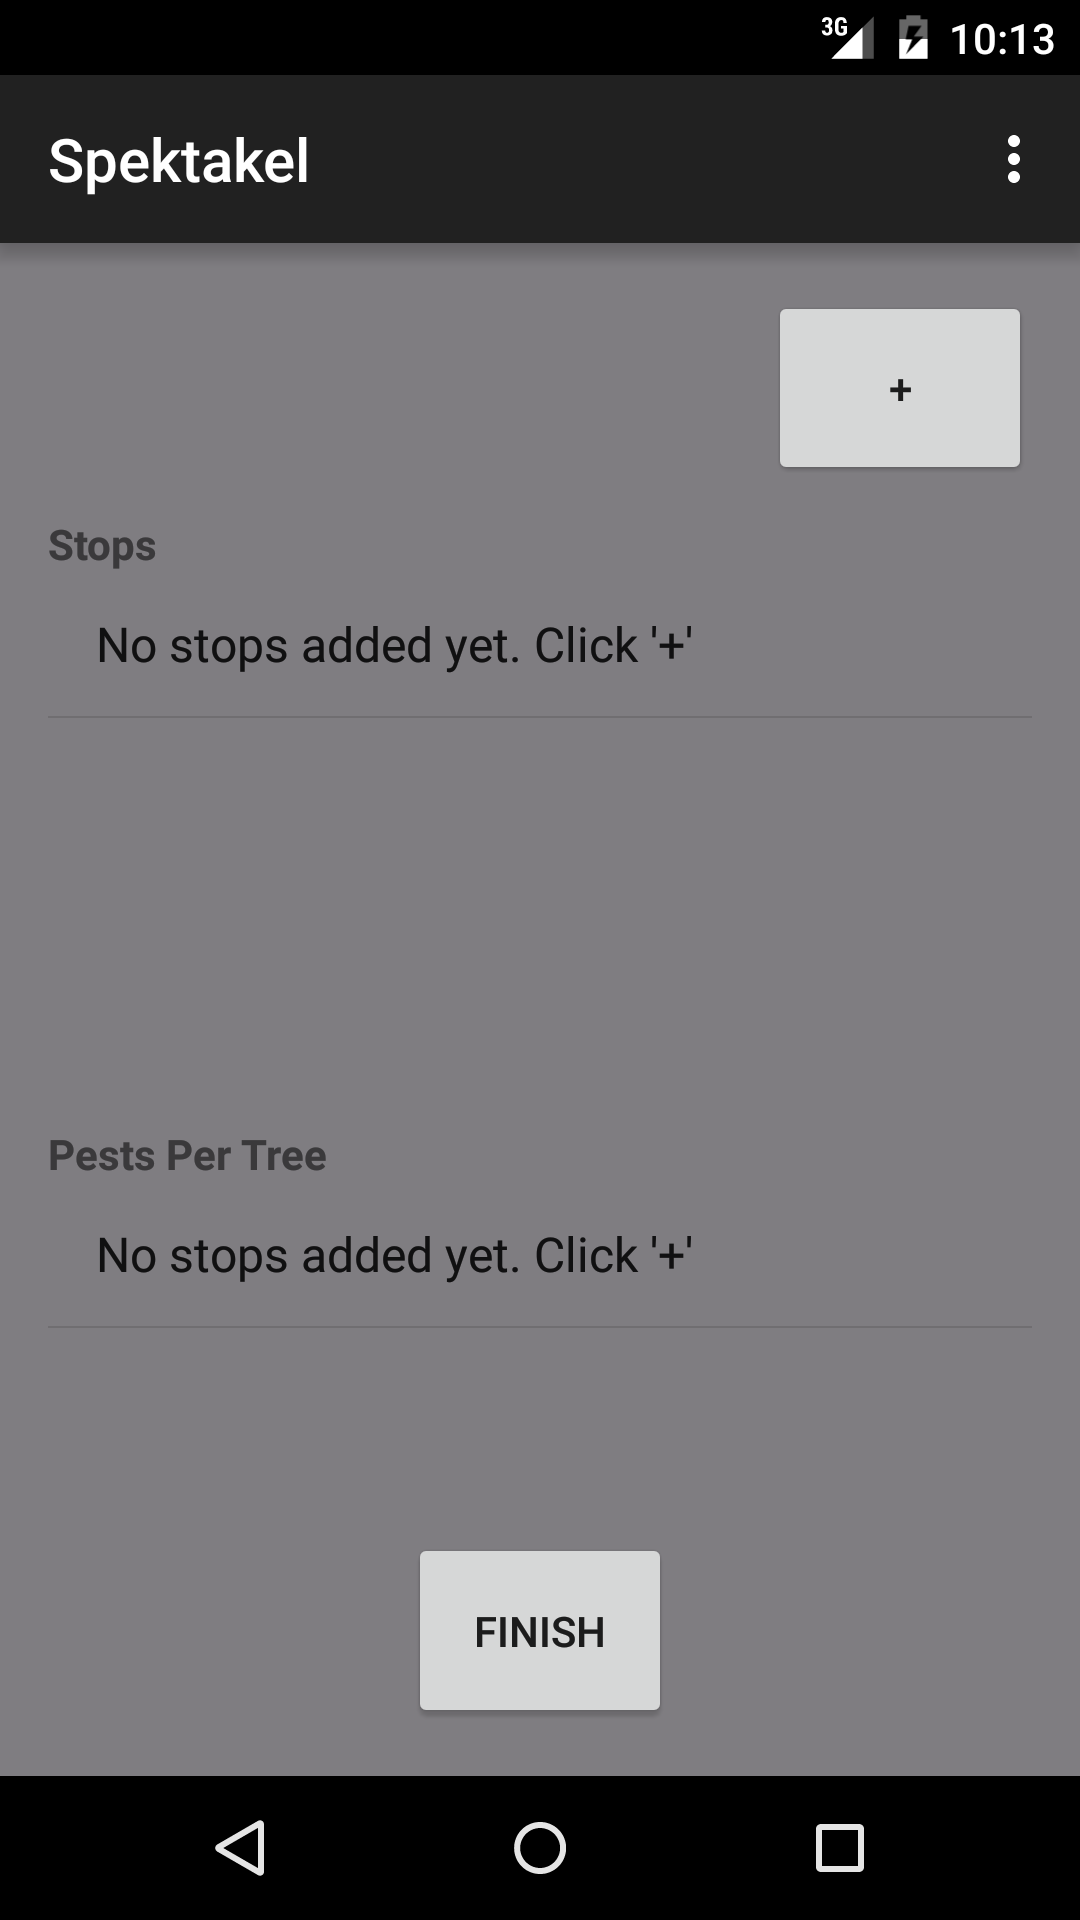
\includegraphics[scale=0.13]{shot2}
			\end{center}
			Click on the [+] button on the top right hand corner of the screen in order to enter new scouting data.

	\item After being directed, select the block in which you are currently situated from the dropdown list at the top. After selecting the block, select the number of trees you have scouted in total. For each individual pile/species of bugs that you have found, select the number of bugs and click on [ADD BUG]. This will redirect you to a different screen in order to identify the specific species of the bug. You will first however be asked to take a photo of the bug.
		\begin{center}
				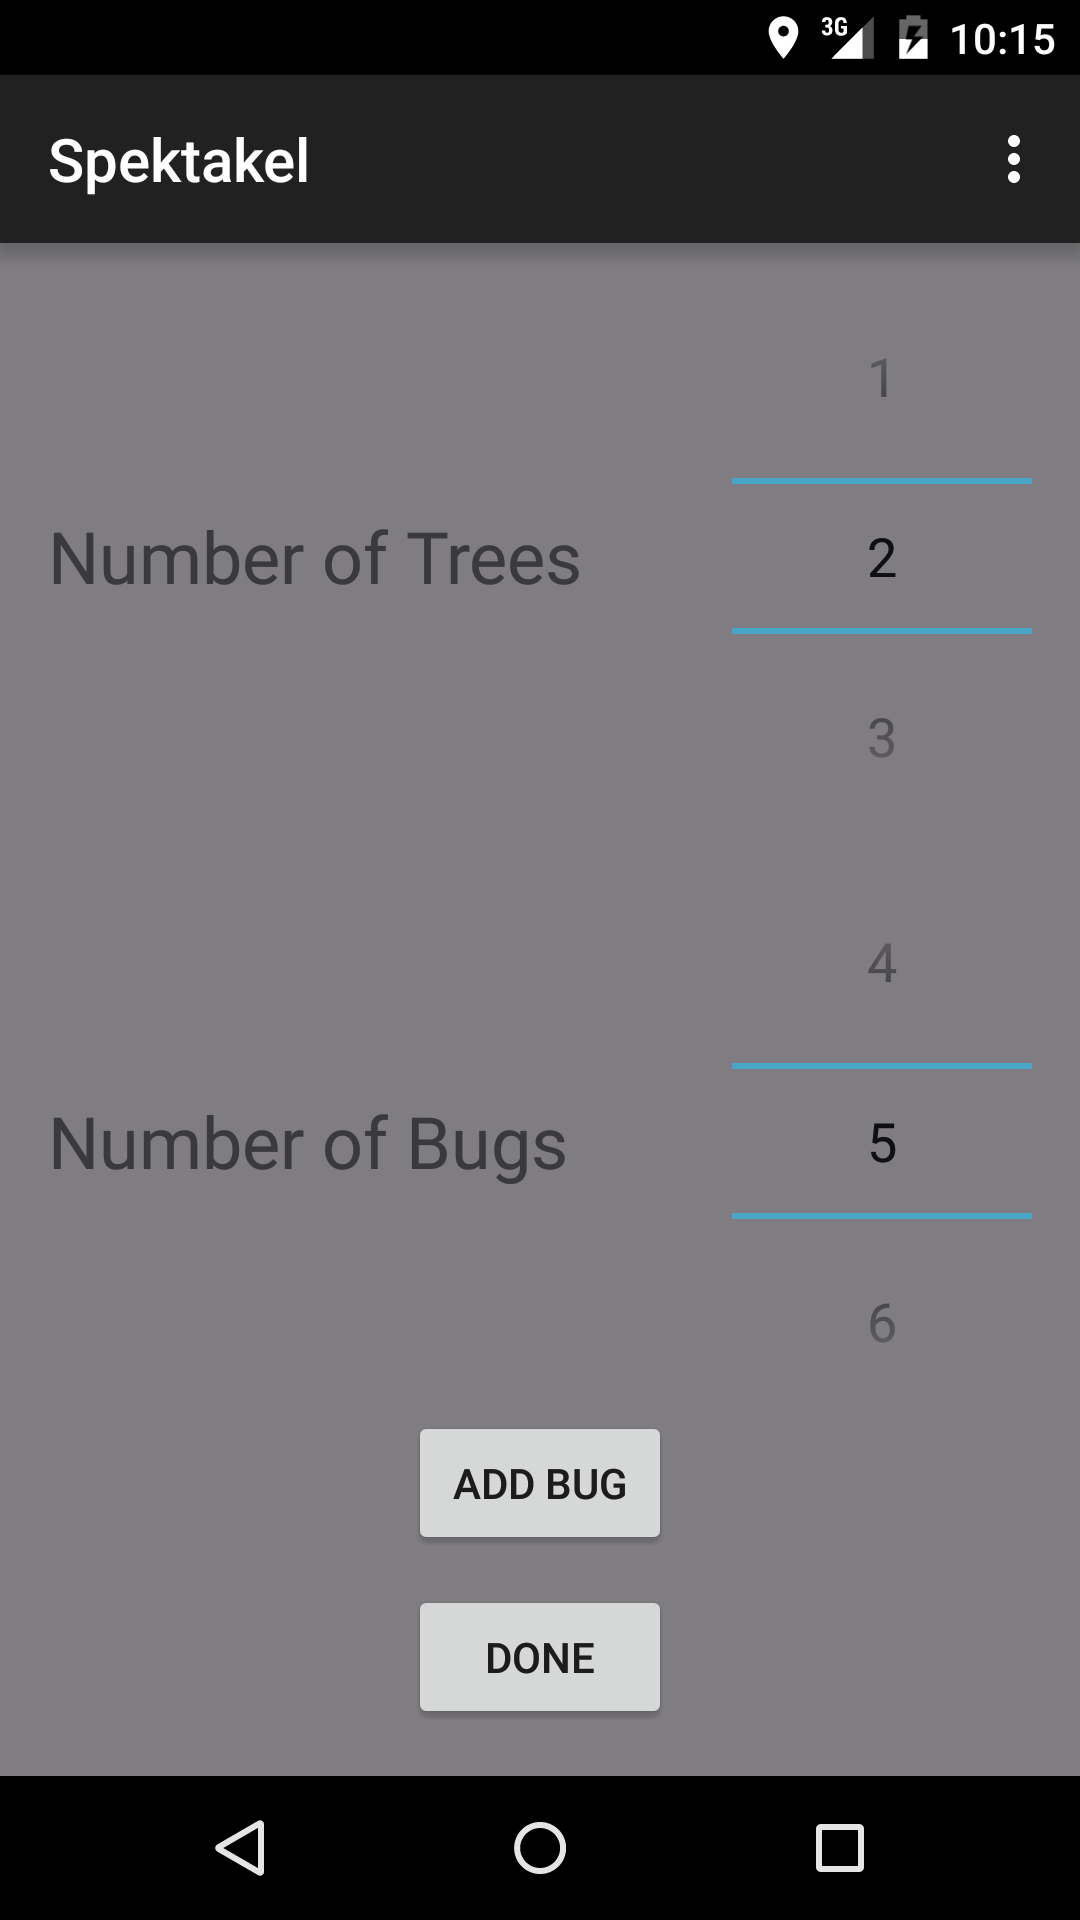
\includegraphics[scale=0.13]{shot3}
			\end{center}

	\item Once a picture of the bug has been taken, your picture will appear on the left hand - top side of the screen. To have the application determine the species automatically, click on the [CHOOSE AUTOMATICALLY] button at the top left corner. If you believe the choice was not accurate or if you prefer to choose the species yourself, select the specific bug type for the gallery from the bottom half of the screen. Once you are satisfied with your selection, click on [DONE].\\
\hfill\\
\textit{NOTE: In the image below the "camera picture" has been replaced with one of the gallery images}
	\begin{center}
				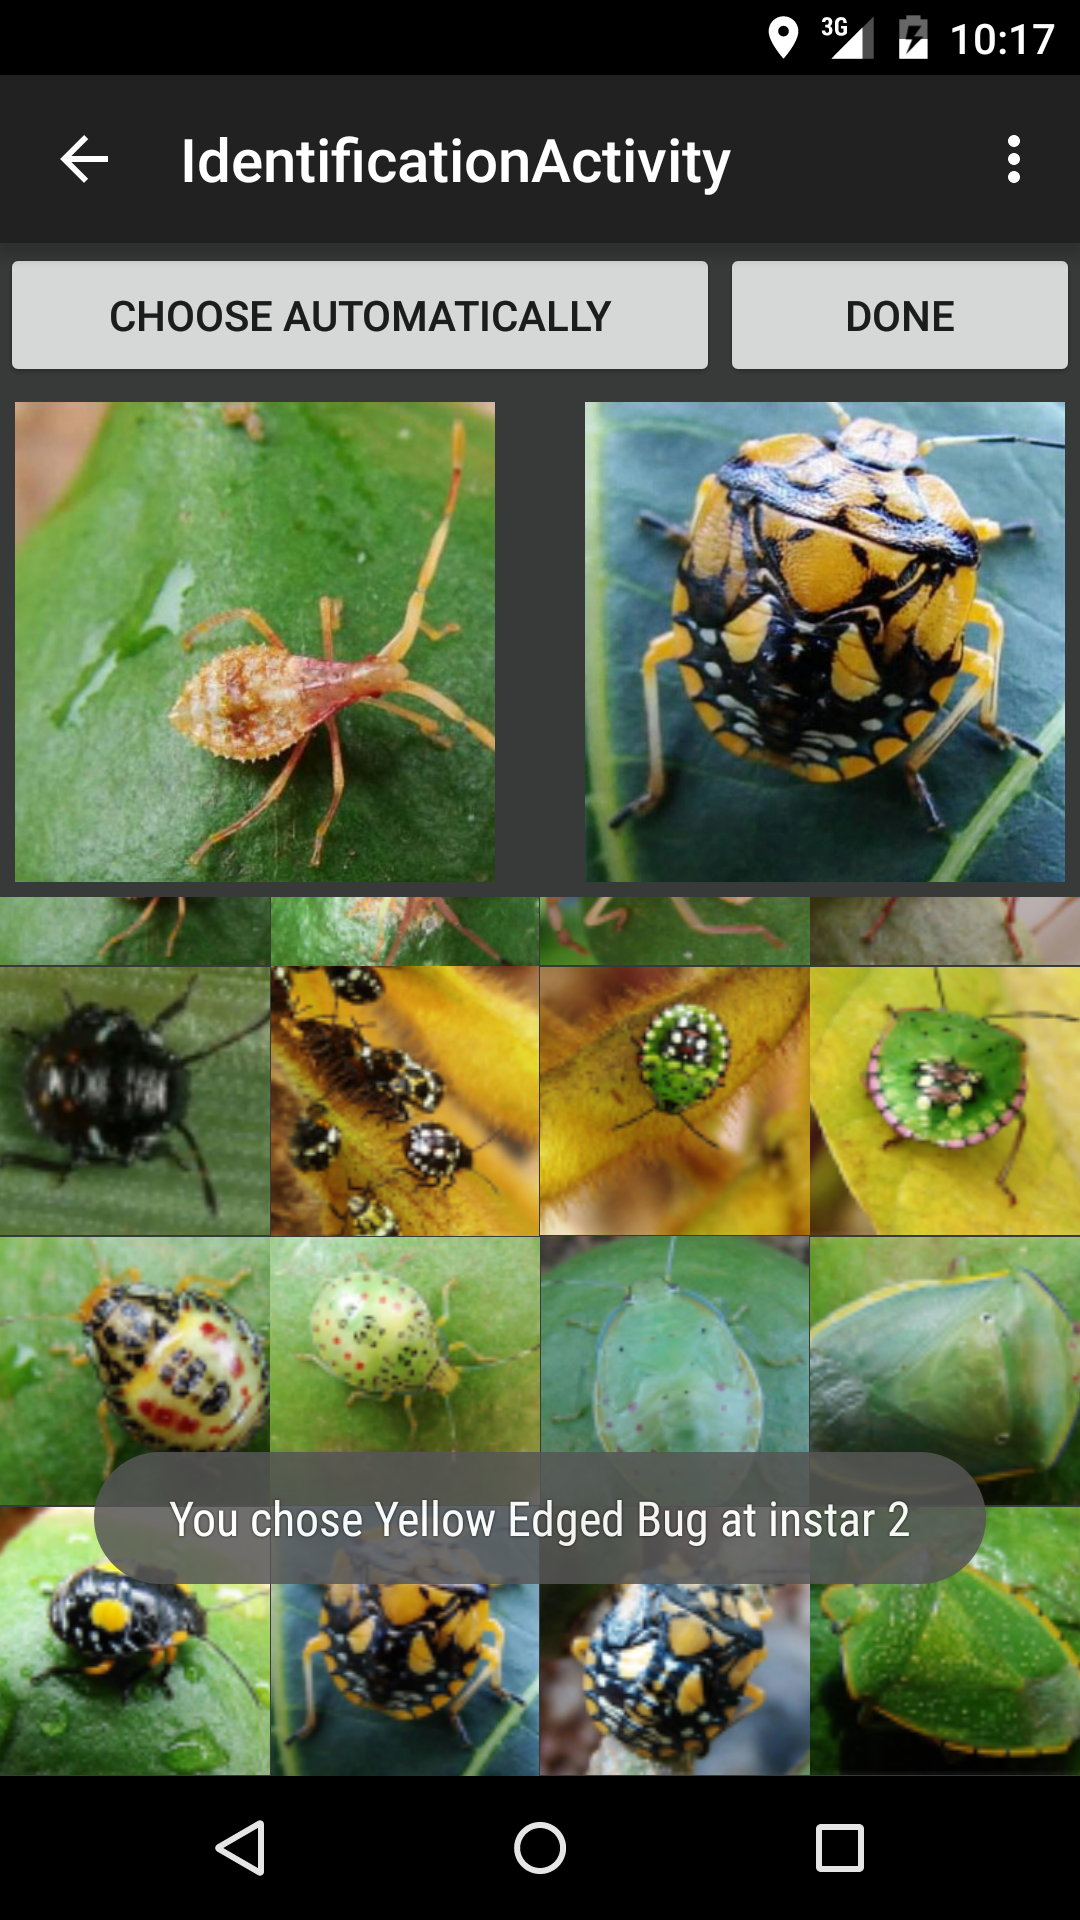
\includegraphics[scale=0.13]{shot4}
			\end{center}

\item Once you are done with selecting the species, repeat steps 4 and 5 until you have identified and counted all the bugs. Your results may look as below for a single entry:

\begin{center}
				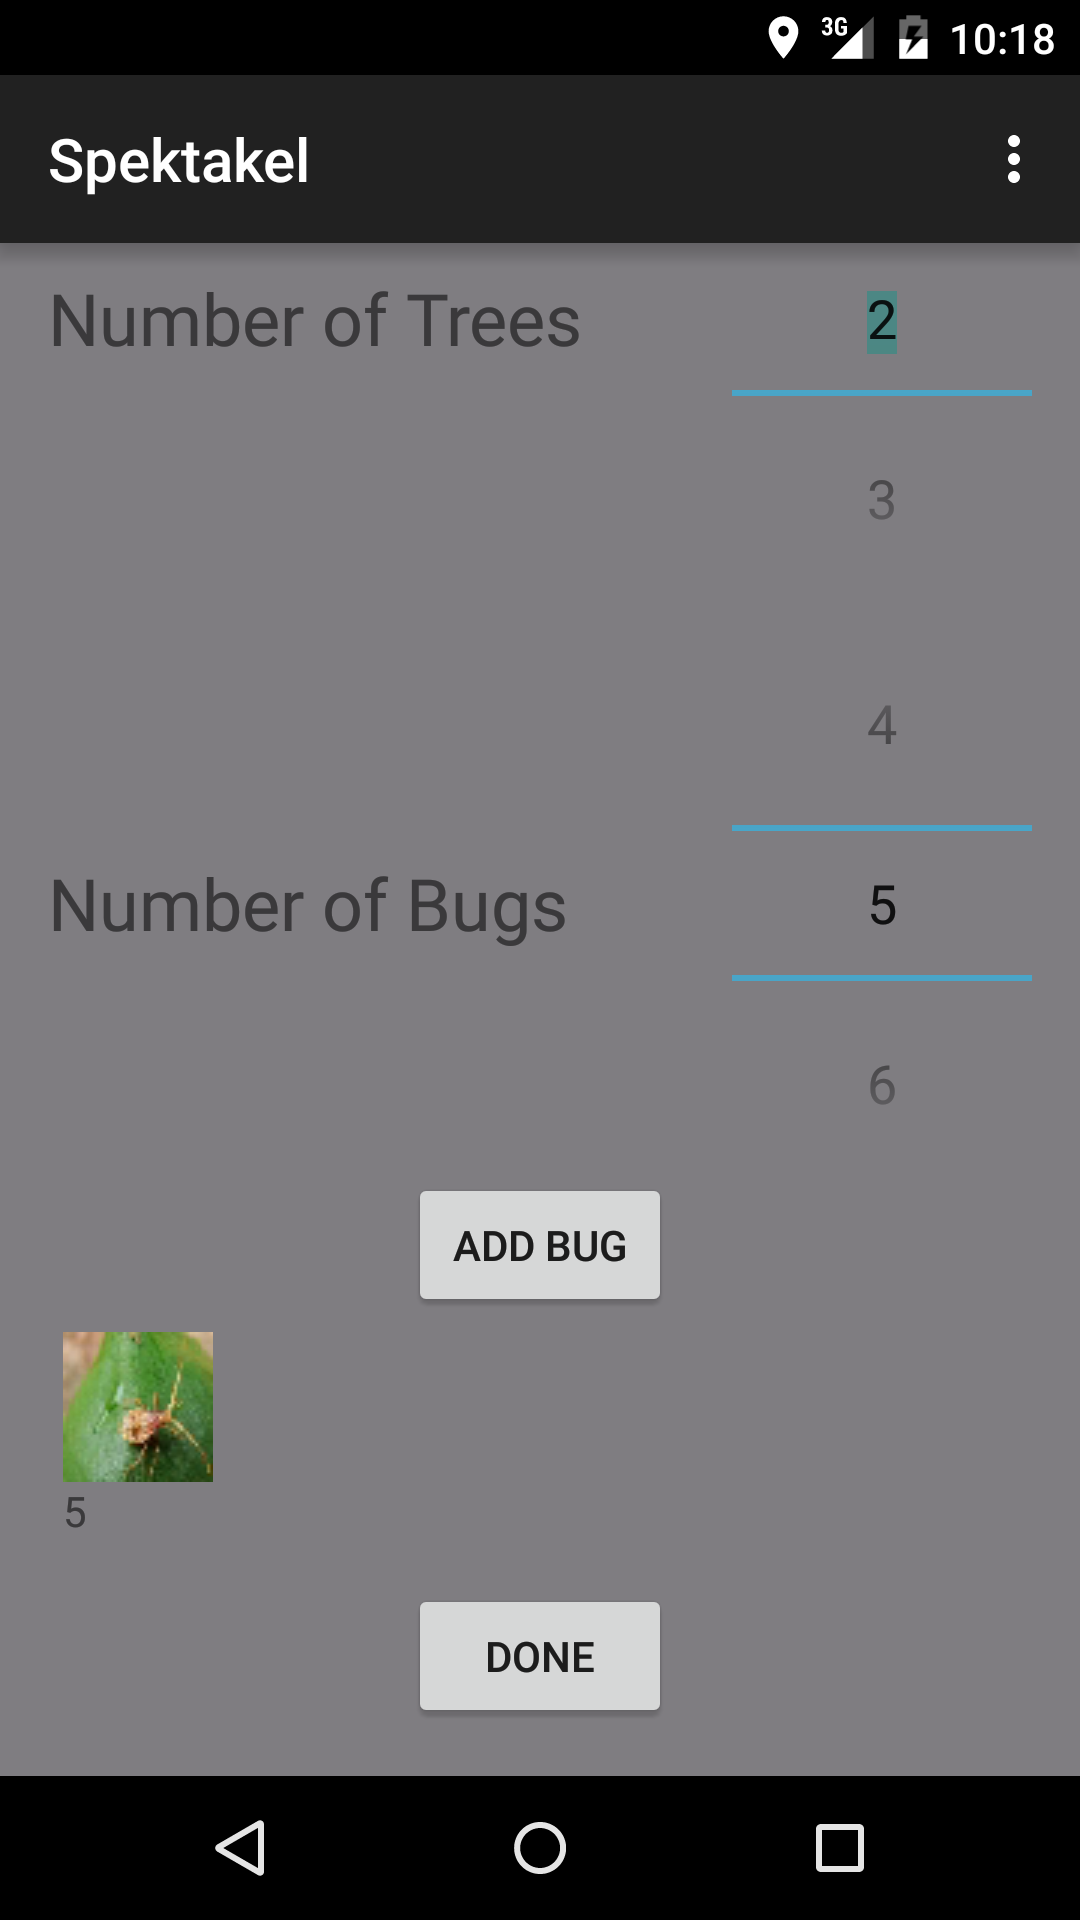
\includegraphics[scale=0.13]{shot5}
			\end{center}

\item When all the bugs have been identified and counted click on [DONE]. You will be directed to a screen showing your scouting information as below:

\begin{center}
				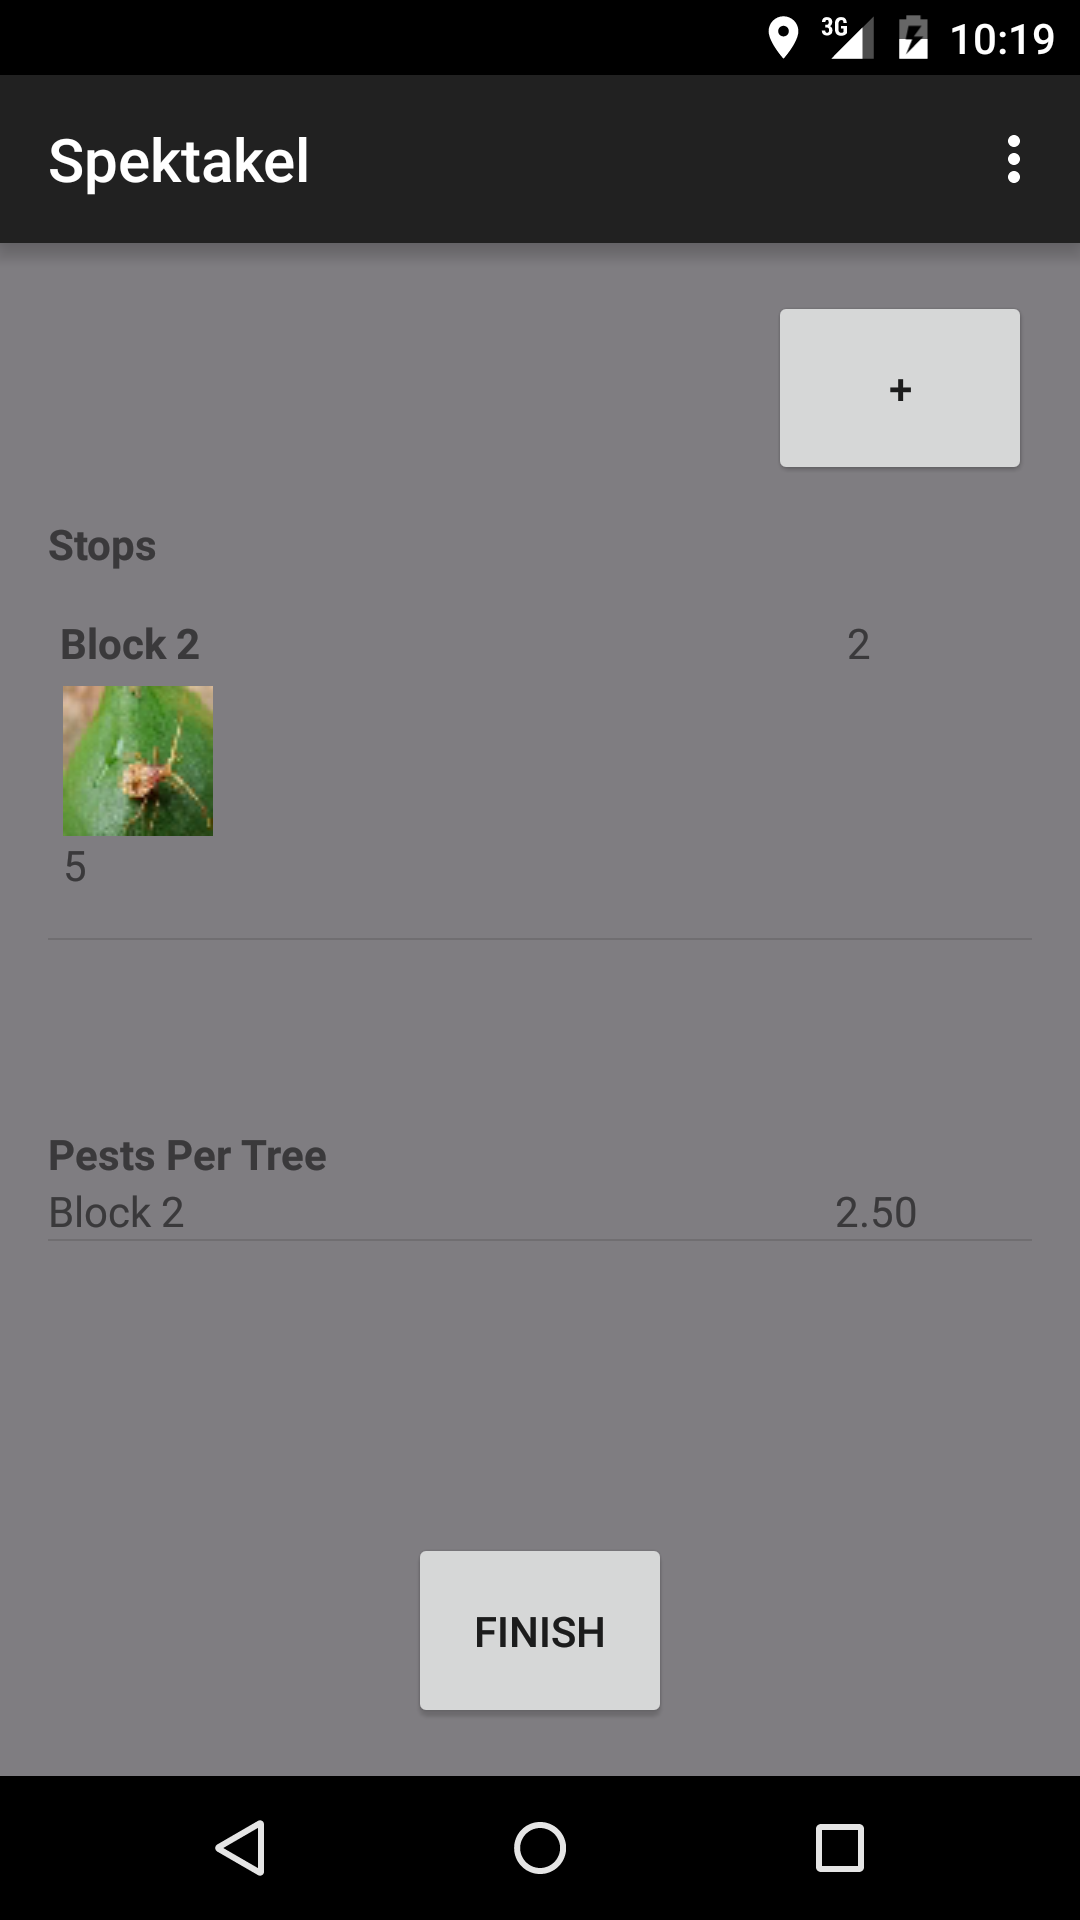
\includegraphics[scale=0.13]{shot6}
\end{center}

\item If you have moved to a different block and/or wish to continue scouting repeat the steps above. When you are done, click [FINISH] and your data will soon be available to the Farmer on the web page.
\end{enumerate}


\section{Troubleshooting}

\end{document}

%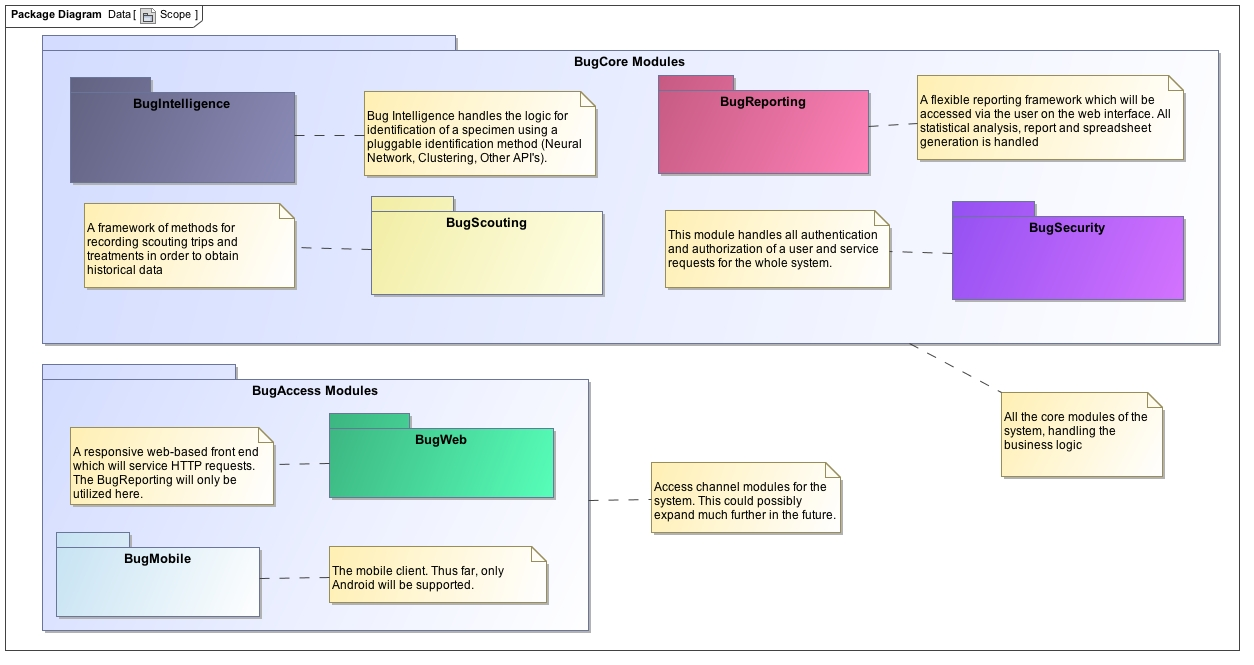
\includegraphics[width=\linewidth]{scope}